\chapter{Estado del Arte}\label{ch:Estado del Arte}
Para la correcta comprensión del trabajo presente, se necesita conocer el estado actual de las herramientas y tecnologías disponibles para el cálculo y la visualización de series de Fourier, así como los estudios y proyectos previos que abordan la implementación de soluciones similares. En este sentido, se revisarán diversas plataformas de uso común que permiten realizar estos procesos de manera separada, además de calcular y/o graficar la serie de Fourier para la función \( f(x) = x \) en el intervalo de \(-\pi\) a \(\pi\) utilizando cada una de las herramientas previamente descritas. El cálculo se realizará en su forma trigonométrica y, en los casos en que la herramienta lo permita, también se obtendrá la forma exponencial compleja. Asimismo, se graficará la serie de Fourier en las plataformas que lo permitan, lo que nos permitirá comparar tanto el proceso como los resultados obtenidos en cada herramienta. \newline

Esta comparación servirá para identificar las capacidades, ventajas y limitaciones de cada una de las plataformas en el contexto del cálculo y la visualización de series de Fourier, evaluando también su facilidad de uso y precisión en la representación gráfica.\newline
\begin{itemize}
	\item \textbf{Forma Trigonométrica}:
	\begin{itemize}
		\item Coeficientes:
		\[
		a_0 = 0, \quad a_n = 0, \quad b_n = \frac{2 (-1)^{n+1}}{n}
		\]
		\item Serie trigonométrica de Fourier para \( f(x) = x \):
		\[
		f(x) = 2 \sum_{n=1}^{\infty} \frac{(-1)^{n+1}}{n} \sin(n x)
		\]
	\end{itemize}
	\item \textbf{Forma Exponencial Compleja}:
	\begin{itemize}
		\item Coeficiente complejo:
		\[
		c_n = \frac{i (-1)^n}{n}, \quad \text{para } n \neq 0.
		\]
		\item Serie exponencial compleja de Fourier para \( f(x) = x \):
		\[
		f(x) = \sum_{\substack{n=-\infty \\ n \neq 0}}^{\infty} \frac{i (-1)^n}{n} e^{i n x}
		\]
	\end{itemize}
\end{itemize}

(Los calculos para llegar a estos coeficientes se encuentran desarrollados en el \hyperref[app:Estado-del-arte-coeff]{Apendice A} .) 

\begin{figure}[h]
	\centering
	\begin{tikzpicture}
		\begin{axis}[
			axis lines=middle,
			grid=both,
			enlargelimits=false,
			width=15cm, % Ancho de la gráfica
			height=13cm, % Altura de la gráfica
			xlabel=$x$,
			ylabel={$f(x)$},
			xtick={-6.28319, -4.7123889, -3.14159, -1.5708, 0, 1.5708, 3.14159, 4.7123889, 6.28319},
			xticklabels={$-2\pi$, $-\frac{3\pi}{2}$, $-\pi$, $-\frac{\pi}{2}$, $0$, $\frac{\pi}{2}$, $\pi$, $\frac{3\pi}{2}$, $2\pi$},
			ymin=-6, ymax=6,
			xmin=-2*pi, xmax=2*pi,
			samples=400,
			domain=-7:7,
			legend style={at={(0.02,0.98)}, anchor=north west},% Posición ajustada a la esquina superior izquierda
			axis background/.style={fill=white}
			]
			
			% Aproximación con 1 término
			\addplot[red, thick] {2*( sin(180*x/pi)/1 )};
			\addlegendentry{Aproximación con 1 término};
			
			% Aproximación con 3 términos
			\addplot[green!70!black, thick] {2*( sin(180*x/pi)/1 - sin(180*2*x/pi)/2 + sin(180*3*x/pi)/3 )};
			\addlegendentry{Aproximación con 3 términos};
			
			% Aproximación con 6 términos
			\addplot[orange, thick] {2*( sin(180*x/pi)/1 - sin(180*2*x/pi)/2 + sin(180*3*x/pi)/3 - sin(180*4*x/pi)/4 + sin(180*5*x/pi)/5 - sin(180*6*x/pi)/6 )};
			\addlegendentry{Aproximación con 6 términos};
			
			% Función Original (línea punteada)
			\addplot[guinda, ultra thick, dashed, domain=-pi:pi] {x};
			\addlegendentry{Función Original};
			
		\end{axis}
	\end{tikzpicture}
	\caption{Gráfica de los coeficientes de Fourier calculados en el \hyperref[app1:Estado-del-arte-coeff]{Apendice A}  \textit{Fuente: Elaboración propia}}
	
	\label{fig:fourier-estado-del-arte}  % Etiqueta para la figura
\end{figure}


Podemos ver en la \ref{fig:fourier-estado-del-arte}, la gráfica de la función y sus aproximaciones de Fourier, donde estas aproximaciones son equivalentes entre la serie trigonométrica y la serie exponencial Esta revisión permitirá contextualizar la propuesta de una aplicación web que integre ambas funcionalidades en una sola plataforma.

\section{Herramientas y Tecnologías Actuales}
Las series de Fourier al formar parte importante en diversas áreas de aprendizaje como la ingeniería, la física y las matemáticas aplicadas, ha impulsado el desarrollo de numerosas soluciones tecnológicas para su cálculo y visualización. En consecuencia, hoy en día disponemos de una gran variedad de plataformas y herramientas que facilitan estos procesos, permitiendo resolver y graficar series de Fourier de forma parcial. En esta sección, se presenta un análisis de las herramientas más significativas para esto, así como sus características, funcionalidades y limitaciones en cuanto a la  incorporación de ambas capacidades en una única plataforma.

\subsection{WolfarmAlpha}
Wolfram Alpha es una aplicación que proporciona respuestas tanto a preguntas como cálculos basados en el motor de Mathematica, un potente software para cálculos simbólicos y numéricos ~\cite{wolframMatemathica}. 
\begin{figure}[H]
	\centering
	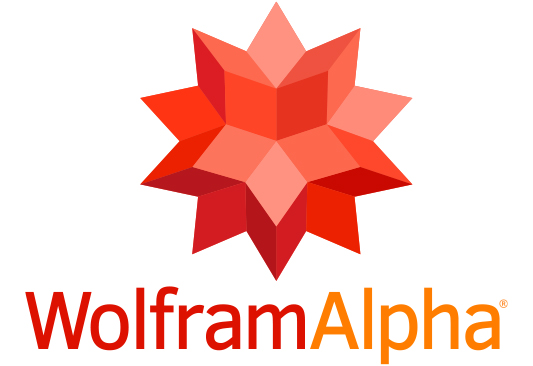
\includegraphics[width=0.5\textwidth]{img/chapter02/logo_wolfram.jpg}
	\caption[Logotipo de WolframAlpha.]{Logotipo de WolframAlpha. \textit{Fuente: ~\cite{wolframMatemathica}}}
	\label{fig:logo-wolfram}  % Etiqueta para la figura
\end{figure}
En contraste con otros motores de búsqueda, en vez de ofrecer una lista de sitios web o documentos, proporciona respuestas precisas y exhaustivas basándose en los conceptos introducidos en su motor de búsqueda. Entre algunas de sus capacidades, este potente software permite tiene funciones propias para resolver y graficar series de Fourier ~\cite{wolfram2024}:
%\begin{itemize}
%	\item \texttt{FourierSeries[exp, t, n]}: Calcula la expansión de la serie de Fourier de la función \texttt{exp} donde esta puede ser de un solo trozo o definida a varios trozos en términos de de la variable \texttt{t} hasta el \texttt{n}.
%	\item \texttt{FourierTrigSeries[exp, t, n]}: Expande en una serie trigonométrica...
%\end{itemize}
\begin{verbatim}
	FourierSeries[exp, t, n]
	FourierTrigSeries[exp, t, n]
	FourierSinSeries[exp, t, n]
	FourierCosSeries[[exp, t, n]]
\end{verbatim} 
Estas funciones nos permiten obtener expansión de la serie de Fourier, ya sea compleja, trigonométrica, en senos o cosenos  de una función \texttt{exp} con periodo de $2\pi$ donde esta puede ser de un solo trozo o definida a varios trozos, para esto se usaría la función \texttt{Piecewise[{{val1,cond1},{val2,cond2},…}]}~\cite{wolframMatemathicaPiecewise}, en términos de de la variable \texttt{t} hasta el \texttt{n}-ésimo término. Además nos mostrará una gráfica estática de una aproximación con \texttt{n} términos. También tiene funciones para calcular los coeficientes de la serie ~\cite{wolframMatemathica}:
\begin{verbatim}
	FourierSeriesCoefficient[exp, t, n]
	FourierSinCoefficient[exp, t, n]
	FourierCosCoefficient[[exp, t, n]]
\end{verbatim} 
Estas funciones nos permiten calcular el \texttt{n}-ésimo coeficiente de la serie de Fourier exponencial compleja, de senos o de cosenos, de una función \texttt{exp} con periodo de $2\pi$, recordando que puede ser a trozos o de un solo trozo. \newline
Podemos observar que las funciones propias de Wolfram Alpha para problemas que impliquen series de Fourier limitan el periodo en el que las funciones matemáticas son definidas, limitándolo en $2*\pi$, para estos casos se podría resolver el coeficiente directamente usando la función de \texttt{Integrate[f,{x,xmin,xmax}]}~\cite{wolframMatemathicaPiecewise} para calcular individualmente cada coeficiente, ya sea $a_0, a_n$ y $b_n$ para las series trigonométricas o $c_0$ y $c_n$ para la serie compleja, pero así no nos proporciona la pequeña gráfica que si nos da al usar las funciones para expandir la serie, además de que la gráfica que se proporciona no es interactiva, y si quieremos verla con más detalle debemos pagar su suscripción.

\subsubsection{Prueba Wolfram Alpha}
Para nuestra primer prueba, calcularemos la serie de Fourier trigonométrica de la función calculada en el  \hyperref[app1:trig-coeff]{Apendice A}, para hacerlo usaremos la función \texttt{FourierTrigSeries(exp, t, n)} de WolframAlpha, que nos permite calcular la serie trigonométrica de Fourier de la función \texttt{exp} respecto a la variable \texttt{t} obteniendo la serie hasta el término \texttt{n}.
\begin{figure}[H]
	\centering
	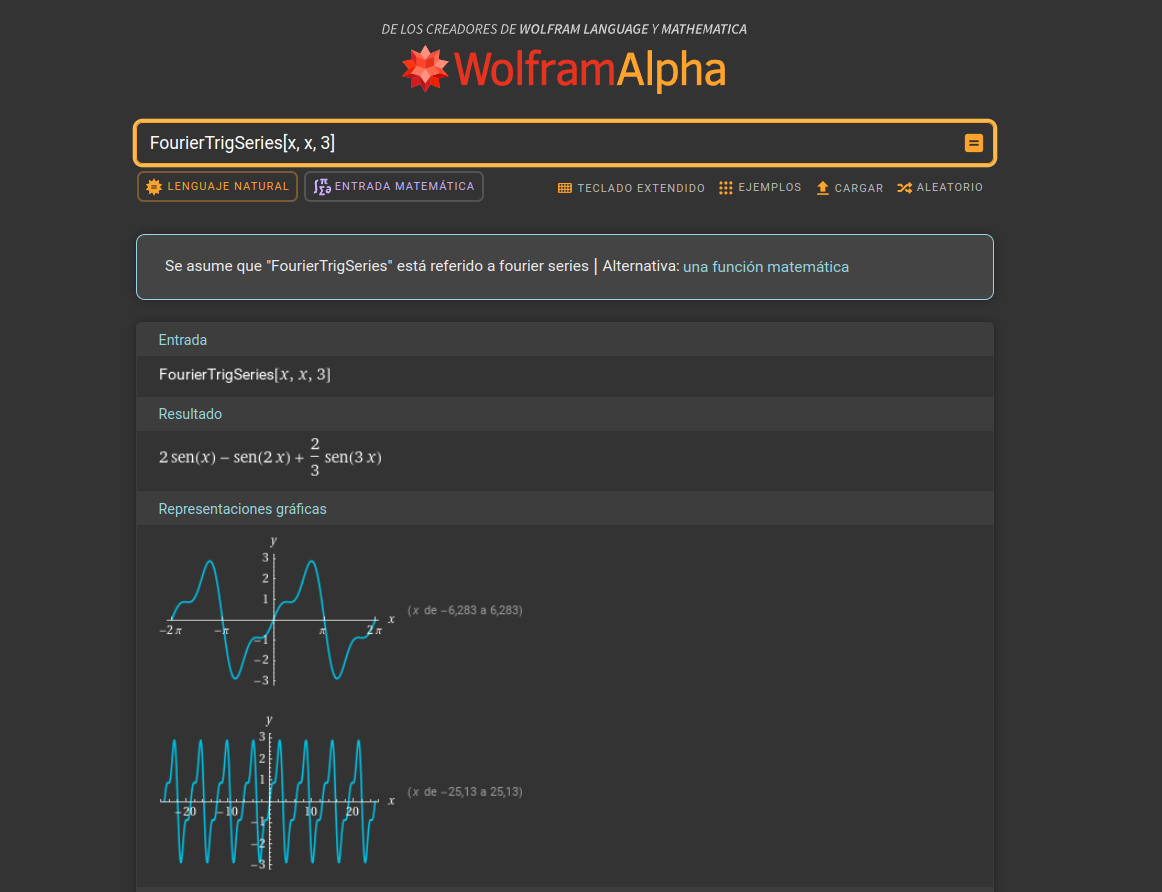
\includegraphics[width=1\textwidth]{img/chapter02/wolfram_trig_series.png}
	\caption{Calculo de una serie trigonométrica de Fourier en WolframAlpha}
	\label{fig:wolfram-trig-series}  % Etiqueta para la figura
\end{figure}
Ahora usaremos la función de \texttt{FourierSeries(exp, t, n)} de WolframAlpha, esta función no permite calcular la serie exponencial compleja de Fourier de la función \texttt{exp} respecto a la variable \texttt{t} obteniendo la serie hasta el término \texttt{n}.
\begin{figure}[H]
	\centering
	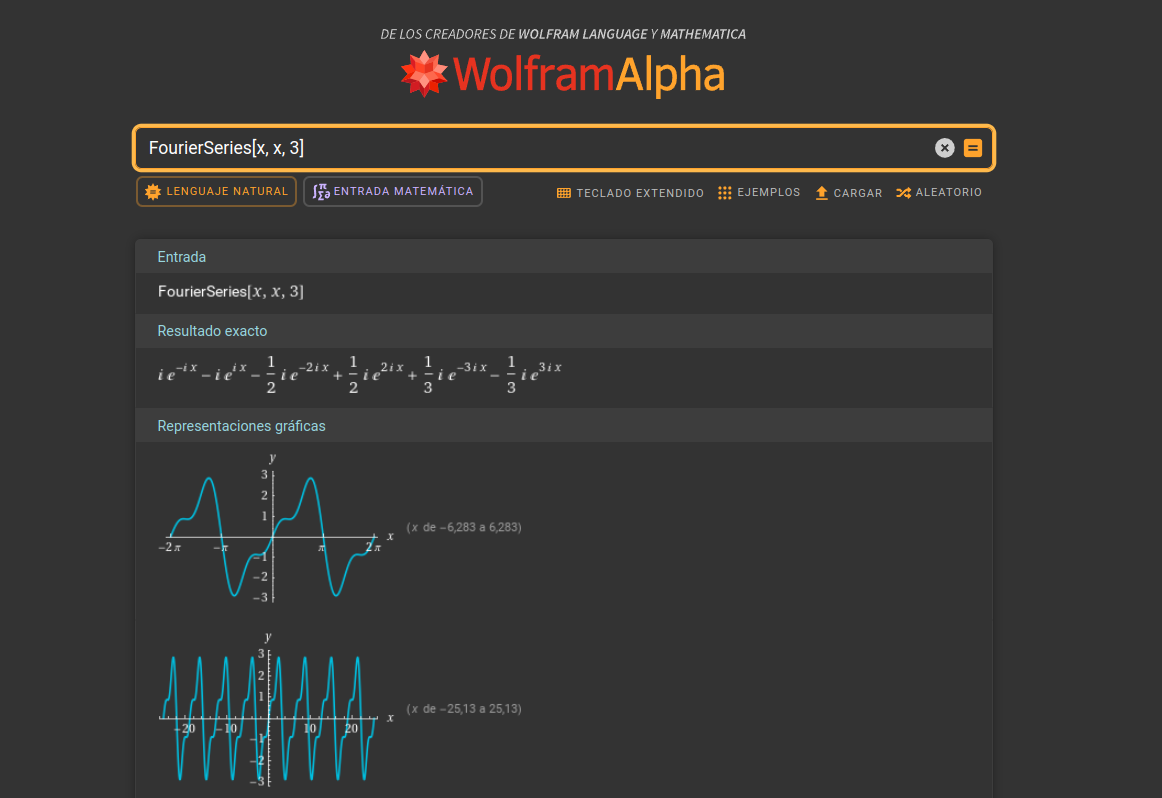
\includegraphics[width=1\textwidth]{img/chapter02/wolfram_complex_series.png}
	\caption{Calculo de una serie trigonométrica de Fourier en WolframAlpha}
	\label{fig:wolfram-exp-series}  % Etiqueta para la figura
\end{figure}
Wolfram nos devuelve la expansión de cada serie en su forma mas reducida, ademas de dos pequeñas gráficas de nuestra aproximación vista desde  no nos devuelve los coeficientes de la serie ni tampoco su expresión final en notación de serie.

\subsection{Symbolab}
Symbolab es una calculadora digital que ayuda a resolver problemas matemáticos, como ecuaciones, álgebra o cálculo. Se trata de una herramienta que puede ser útil para aprender matemáticas, ya que ofrece evaluaciones personalizadas y conocimientos impulsados por inteligencia artificial. ~\cite{symbolabDocs}. 
\begin{figure}[H]
	\centering
	
\includegraphics[width=0.3\textwidth]{img/chapter02/logo_symbolab.png}
	\caption[Logotipo de Symbolab.]{Logotipo de Symbolab. \textit{Fuente: ~\cite{symbolabDocs}}}
	\label{fig:logo-symbolab}  % Etiqueta para la figura
\end{figure}
Symbolab se centra en la enseñanza de procedimientos matemáticos mediante explicaciones detalladas. Su interfaz es especialmente útil para estudiantes, ya que presenta guías paso a paso para temas como derivadas, integrales y ecuaciones algebraicas complejas, lo cual es ideal para el aprendizaje autodidacta. Este cuenta con una función para resolver series de Fourier en su forma trigonométrica denominada \texttt{fourier series (f), [-L, L]} ~\cite{symbolabDocs} en donde \texttt{f} es una función definida en el intervalo de \texttt{[-L, L]}. A pesar de contar con funciones para definir funciones matemáticas a trozos y funciones para hacer gráficas, no es posible unificarlas en la misma aplicación, ademas de no contar con funciones para otras series de Fourier como extensiones de medio rango o exponencial compleja, pero, al igual que en Wolfram Alpha, se pueden calcular individualmente los coeficientes con la función \texttt{integral from a to b of x}~\cite{symbolabDocs}.

\subsubsection{Prueba Symbolab}
Para nuestra siguiente prueba, calcularemos la serie de Fourier trigonométrica de de la función calculada en el \hyperref[app1:trig-coeff]{Apendice A}, para hacerlo usaremos la función \texttt{fourier series (f), [-L, L]} de Symbolab, que nos permite calcular la serie trigonométrica de Fourier de la función \texttt{f} respecto a la variable obteniendo desde el intervalo \texttt{-L} a \texttt{L}.
\begin{figure}[H]
	\centering
	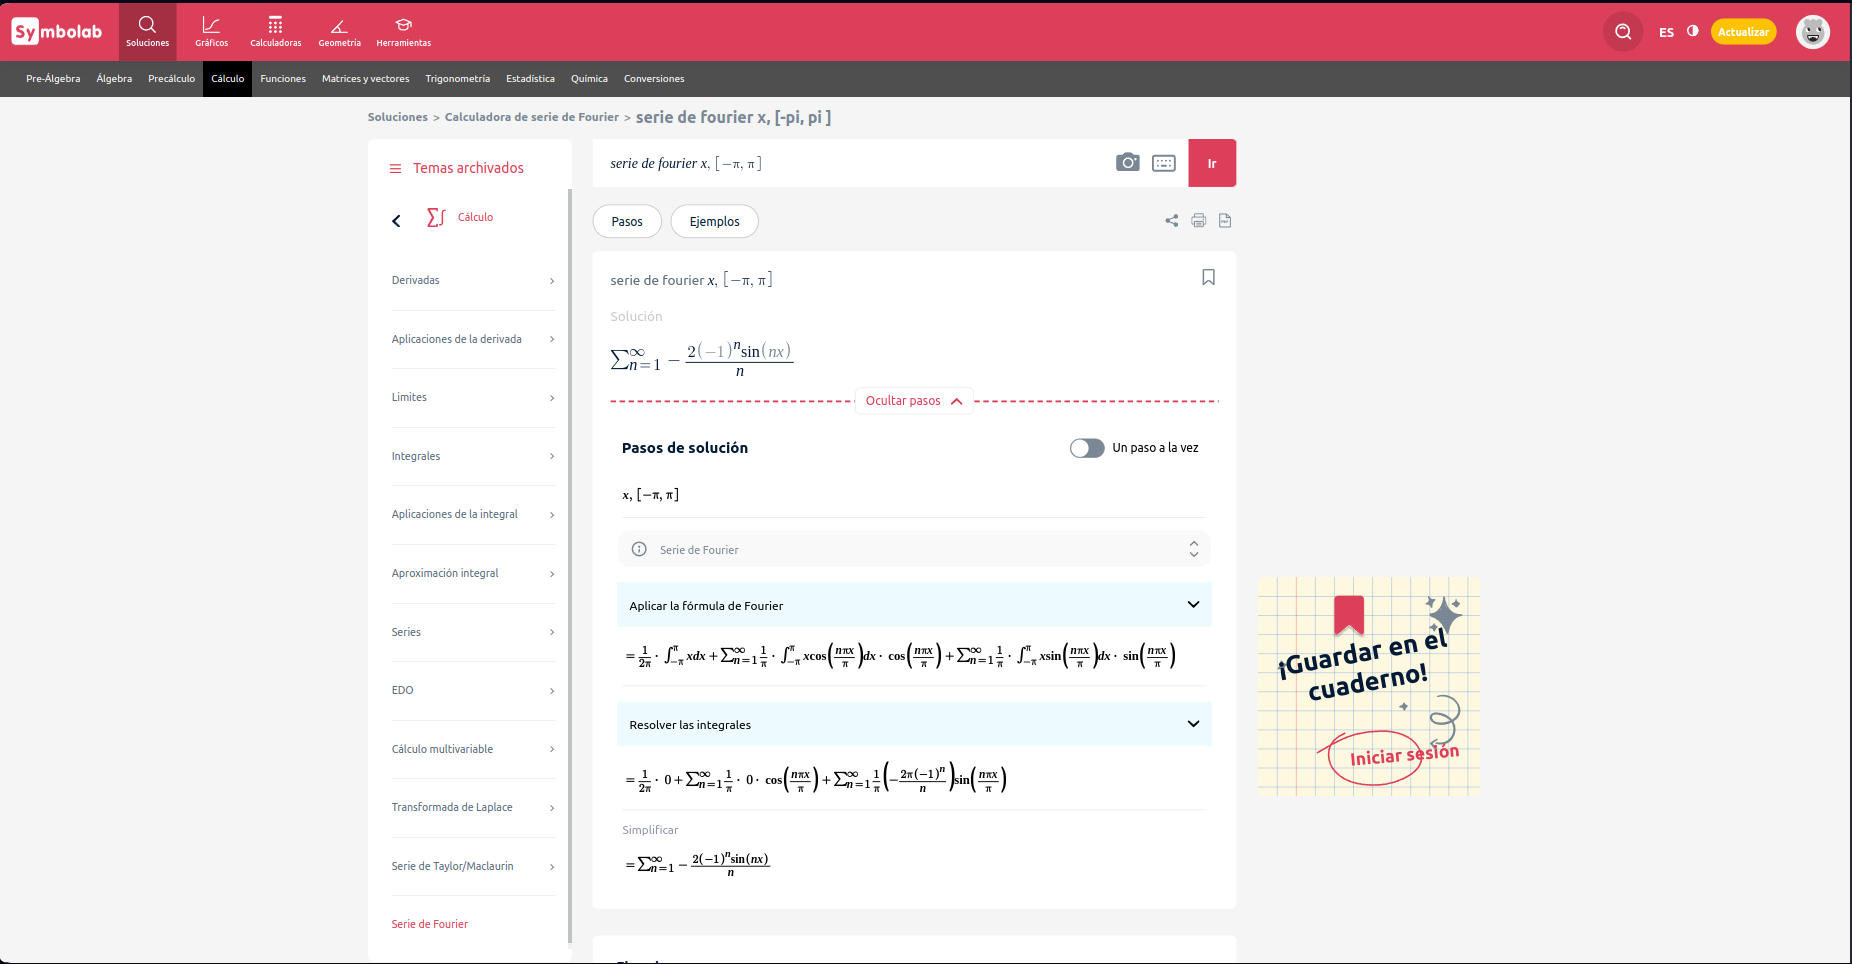
\includegraphics[width=1\textwidth]{img/chapter02/symbolab-trig-series.png}
	\caption{Calculo de una serie trigonométrica de Fourier en Symbolab}
	\label{fig:symbolab-trig-series}  % Etiqueta para la figura
\end{figure}
Symbolab nos dará la expresión en forma de serie, y solo podremos hacerlo para la serie trigonométrica, ademas de que no nos muestra ninguna gráfica.

\subsection{MATLAB} 
MATLAB es un entorno de programación y un lenguaje de alto nivel ampliamente utilizado en ingeniería, física y matemáticas aplicadas para el análisis numérico, la visualización de datos y el desarrollo de algoritmos. Su robusta caja de herramientas, especialmente la \textit{Signal Processing Toolbox} y la \textit{Symbolic Math Toolbox}, facilitan el cálculo y la graficación de series de Fourier  ~\cite{MathWorks2024}.

\begin{figure}[H]
	\centering
	
\includegraphics[width=0.5\textwidth]{img/chapter02/logo_matlab.png}
	\caption[Logotipo de Matlab.]{Logotipo de Matlab. \textit{Fuente: ~\cite{MathWorks2024}}}
	\label{fig:logo-matlab}  % Etiqueta para la figura
\end{figure}

A pesar de que MATLAB cuenta con funciones especiales para el análisis de Fourier como la transformada de Fourier (\texttt{fourier(f)}) o la Transformada rápida de Fourier (\texttt{fft(f)}) no cuenta con funciones especificas para series de Fourier, sin embargo, podemos definir nuestros coeficientes para hacer el gráfico de ambas series.

\subsubsection{Prueba Matlab}
Para la prueba con Matlab, primero ejecutaremos el código en \hyperref[app2:trig-code-matlab]{Apendice B}, que nos graficará la serie de Fourier a partir de sus coeficientes trigonométricos \ref{fig:matlab-trig-series}. 
\begin{figure}[H]
	\centering
	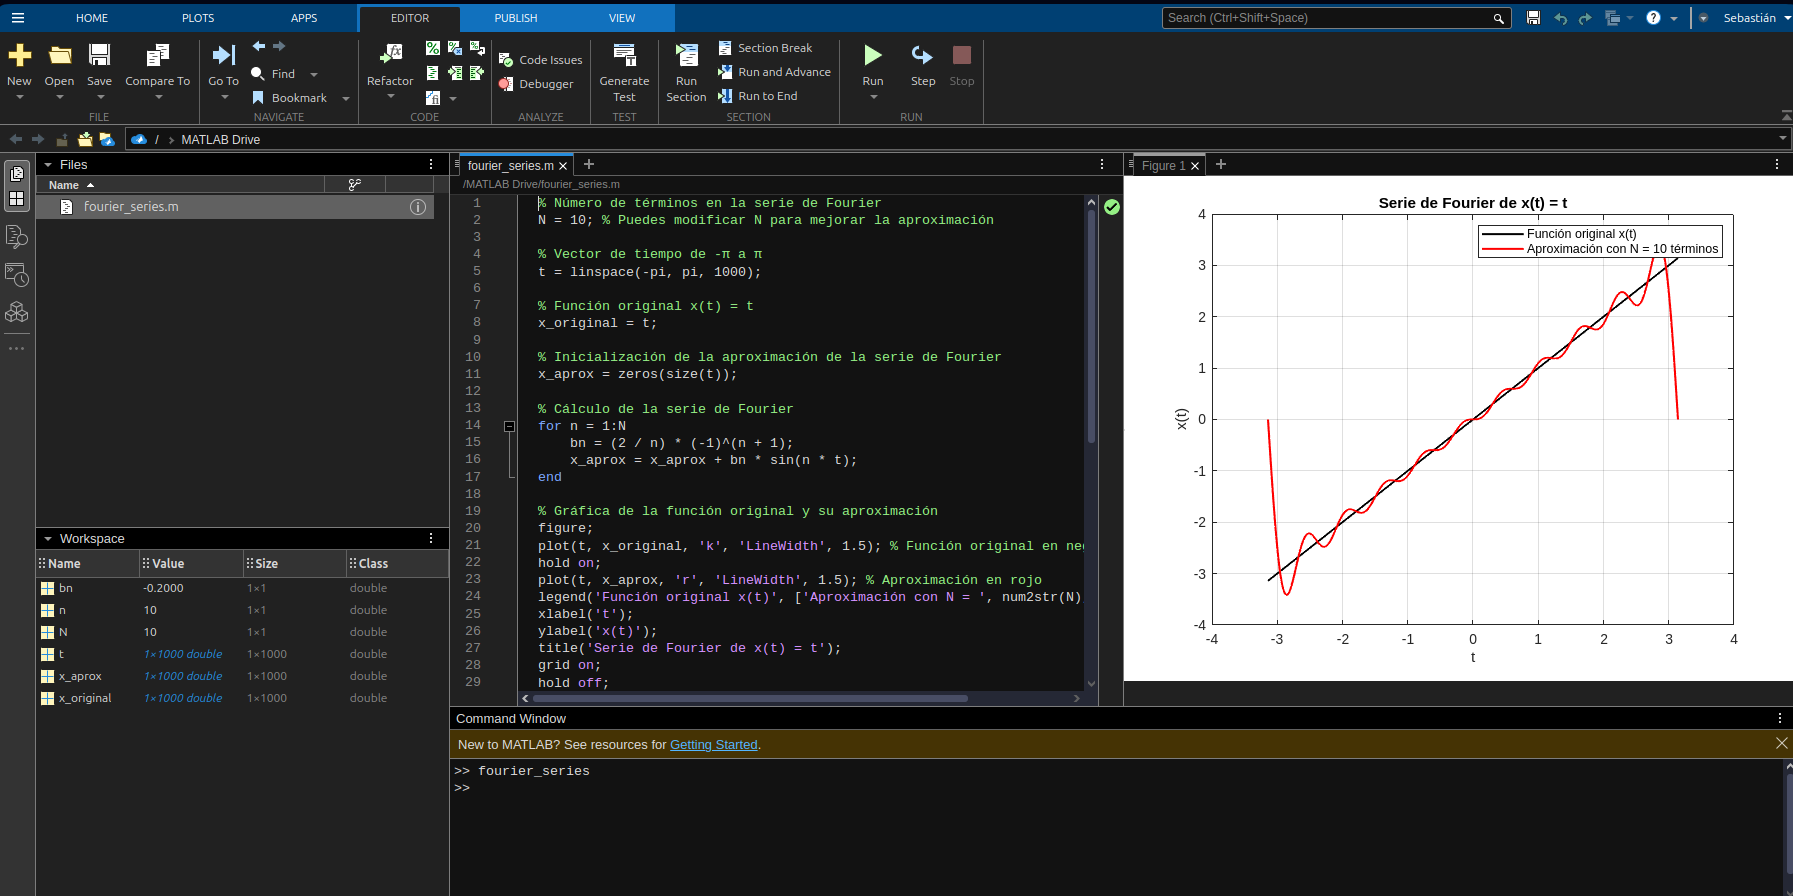
\includegraphics[width=1\textwidth]{img/chapter02/matlab-fourier-trig.png}
	\caption{Graficación de una serie trigonométrica de Fourier en Matlab}
	\label{fig:matlab-trig-series}  % Etiqueta para la figura
\end{figure}
Ahora usamos el código en \hyperref[app2:complex-code-matlab]{Apendice B} para graficar la misma serie pero ahora usando su coefciente complejo \ref{fig:matlab-complex-series}.
\begin{figure}[H]
	\centering
	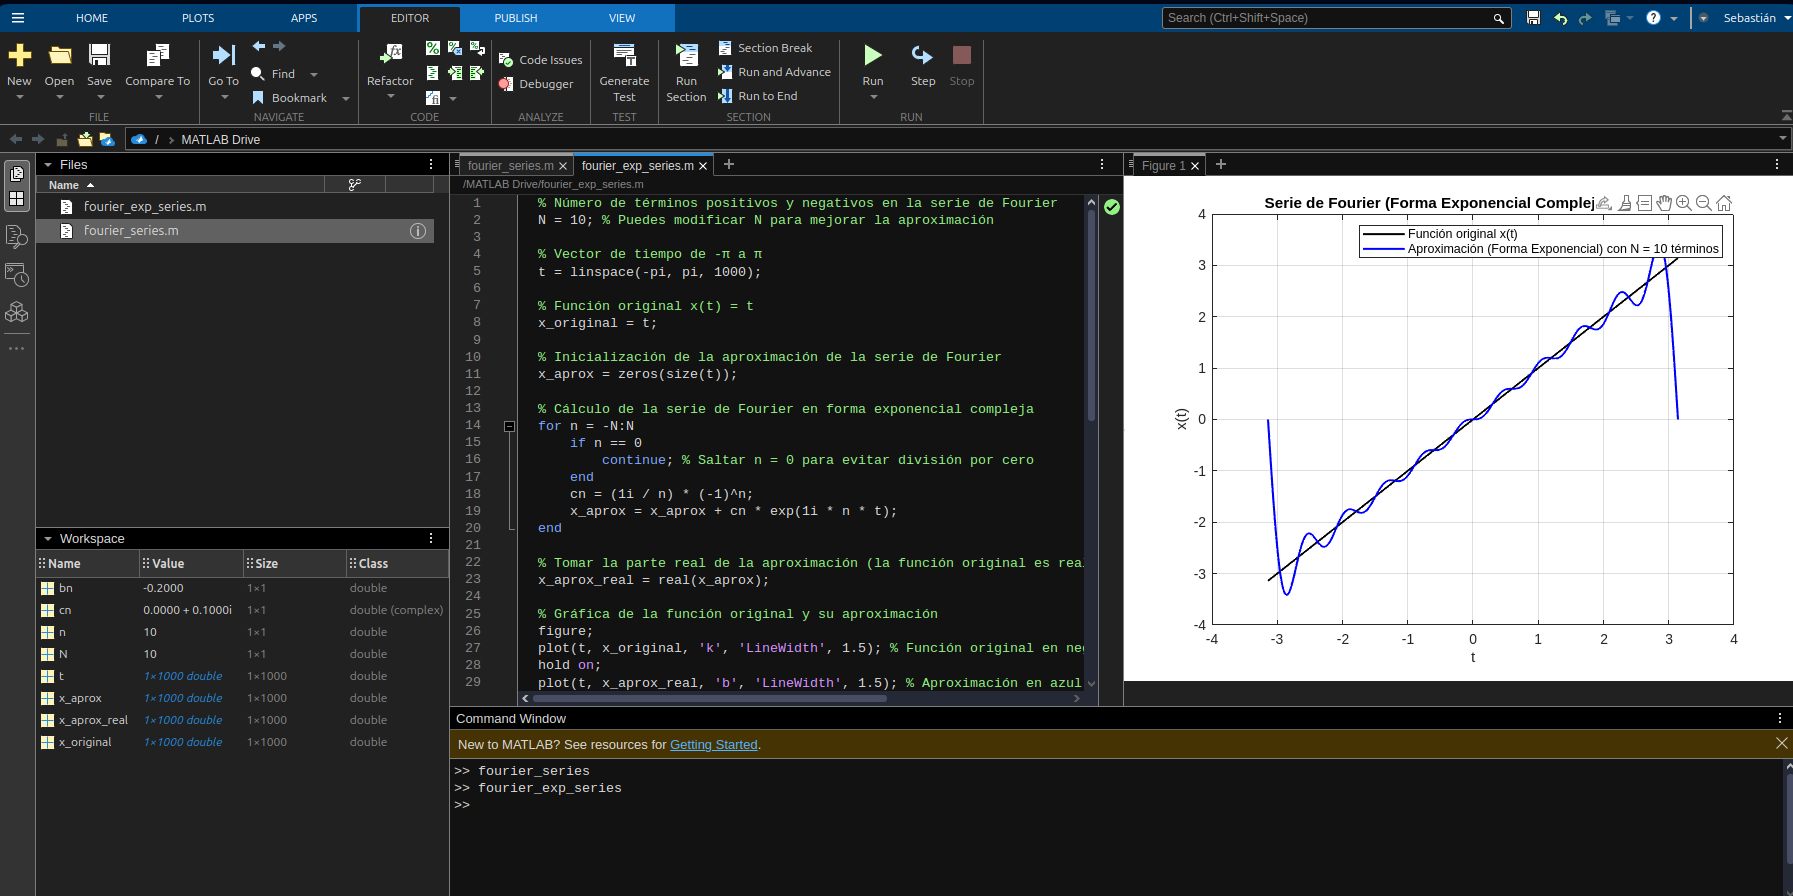
\includegraphics[width=1\textwidth]{img/chapter02/matlab-complex-series.png}
	\caption{Graficación de una serie compleja de Fourier en Matlab}
	\label{fig:matlab-complex-series}  % Etiqueta para la figura
\end{figure}
Matlab es capaz de graficar muy buenas aproximaciones de ambas series en una gráfica que nos brinda cierto nivel de interactividad pero todo dependerá de nuestros cálculos y de que tanto detalle plasmemos en nuestro código para aumentar las funcionalidades

\subsection{Maple}
Python es un lenguaje de programación ampliamente utilizado en las aplicaciones web, el desarrollo de software, la ciencia de datos y el machine learning (ML). Los desarrolladores utilizan Python porque es eficiente y fácil de aprender, además de que se puede ejecutar en muchas plataformas

\subsection{Maxima}
Python es un lenguaje de programación ampliamente utilizado en las aplicaciones web, el desarrollo de software, la ciencia de datos y el machine learning (ML). Los desarrolladores utilizan Python porque es eficiente y fácil de aprender, además de que se puede ejecutar en muchas plataformas

\subsection{Geogebra / Desmos}
Python es un lenguaje de programación ampliamente utilizado en las aplicaciones web, el desarrollo de software, la ciencia de datos y el machine learning (ML). Los desarrolladores utilizan Python porque es eficiente y fácil de aprender, además de que se puede ejecutar en muchas plataformas

\subsection{Python}
Python es un lenguaje de programación ampliamente utilizado en las aplicaciones web, el desarrollo de software, la ciencia de datos y el machine learning (ML). Los desarrolladores utilizan Python porque es eficiente y fácil de aprender, además de que se puede ejecutar en muchas plataformas diferentes. El software Python se puede descargar gratis, se integra bien a todos los tipos de sistemas y aumenta la velocidad del desarrollo ~\cite{amazonPython}.
La versatilidad de python permiten que se creen librerías para todo tipo de tareas con él, una de ellas es la de hacer cálculos matemáticos y creación de gráficos, de los cuales, podemos tomar funciones especificas para ayudarnos en el calculo de series de Fourier

\subsubsection{Sympy / Matplotlib}
Python es un lenguaje de programación ampliamente utilizado en las aplicaciones web, el desarrollo de software, la ciencia de datos y el machine learning (ML). Los desarrolladores utilizan Python porque es eficiente y fácil de aprender, además de que se puede ejecutar en muchas plataformas diferentes. El software Python se puede descargar gratis, se integra bien a todos los tipos de sistemas y aumenta la velocidad del desarrollo.

\subsubsection{Manim}
Python es un lenguaje de programación ampliamente utilizado en las aplicaciones web, el desarrollo de software, la ciencia de datos y el machine learning (ML). Los desarrolladores utilizan Python porque es eficiente y fácil de aprender, además de que se puede ejecutar en muchas plataformas diferentes. El software Python se puede descargar gratis, se integra bien a todos los tipos de sistemas y aumenta la velocidad del desarrollo.

\section{Comparativa del Funcionamiento de las Herramientas}

\begin{longtable}{ | m{2.5cm} | m{6.5cm} | m{4cm} | }
	\rowcolor{black!75}
	\head {SOFTWARE} & \head {CARACTERÍSTICAS} & \head {PRECIO} \\ \hline
	\endfirsthead
	\multicolumn{3}{c}{{\tablename\ \thetable{} -- continuación}} \\
	\rowcolor{black!75}
	\head {SOFTWARE} & \head {CARACTERÍSTICAS} & \head {PRECIO} \\ \hline
	\endhead
	\hline \multicolumn{3}{r}{{Continúa en la siguiente página}} \\
	\endfoot
	\hline
	\endlastfoot
	Wolfram Alpha & Se trata de un potente motor comercial de conocimiento computacional para cálculos matemáticos y gráficos. Contiene módulos que permiten el calculo de los coeficientes de Series de Fourier (Trigonométrica y compleja) así como las extensiones pares e impares para funciones simples o a trozos, así como poder expandir la serie y obtener una gráfica estática.~\cite{wolfram2024}  & Desde MXN \$1,200.00 anuales para estudiantes, plan gratuito limitado. \\ \hline
	Geogebra & Herramienta dinámica para construcciones geométricas y gráficas. Podemos graficar cualquier serie o extensión trigonométrica y poder ver como cambia la serie conforme añadimos más coeficientes. Requiere que hagamos los cálculos y armar la expresión de la serie~\cite{GeoGebra2024} & Software libre y código abierto \\ \hline
	Desmos  & Similar a Geogebra es una calculadora gráfica en línea para cálculos y gráficos, donde de igual modo podemos graficar cualquier serie o extensión trigonométrica y poder ver como cambia la serie conforme añadimos más coeficientes. Requiere cálculos previos para series de Fourier.~\cite{Desmos2024} & Software libre y código abierto\\ \hline
	Python$_{Manim}$ & Librería de animación en Python para visualizaciones matemáticas, incluida la animación de series de Fourier. Podemos graficar cualquier serie ya sea trigonométrica o exponencial y poder animar de infinitas maneras el como se aproxima la serie con sus coeficientes. Requiere hacer los cálculos, armar la expresión de la serie y tener conocimientos en Python, programación orientada a objetos y a librería de Manim ~\cite{Manim2024} & Software libre y código abierto \\ \hline
	Python$_{SymPy}$ &Es una biblioteca de Python para realizar matemáticas simbólicas, que incluye el cálculo de series de Fourier. A menudo se usa en combinación con librerías de visualización como Matplotlib para representar gráficamente los resultados, pero de nuevo, esta combinación requiere conocimientos de programación.~\cite{Matplotlib-sympy2024} & Software libre y código abierto \\ \hline
	Matlab  & Es un entorno de programación comercial para cálculos numéricos y visualización de datos, con herramientas específicas para series de Fourier, además de tener funciones para poder graficarlas. Requiere conocimientos en matlab.~\cite{MathWorks2024} & Desde USD\$99 (aprox. MXN\$1627.82) anuales para estudiantes.\\ \hline	
	\rowcolor{white}\caption{Comparación de software para cálculos matemáticos y visualización de datos} \label{tabla:software} \\
\end{longtable}

\section{Trabajos y Proyectos Relacionados}
En esta sección se analizarán trabajos académicos y proyectos de investigación que han desarrollado herramientas similares o que abordan la enseñanza de series de Fourier y el uso de plataformas interactivas para la educación matemática. 

%\begin{table}[h]
%	\centering
%	\begin{tabular}{ | m{2.5cm} | m{6.5cm} | m{4cm} | }
%		\rowcolor{black!75}
%		\head {SOFTWARE} & \head {CARACTERÍSTICAS} & \head {PRECIO} \\ \hline
%		Wolfram Alpha & Potente motor de conocimiento computacional para cálculos matemáticos y gráficos. No especializado en series de Fourier.~\cite{wolfram2024}  & Desde MXN \$1,200.00 anuales para estudiantes, plan gratuito limitado. \\ \hline
%		Geogebra & Herramienta dinámica para construcciones geométricas y gráficas. Requiere cálculos previos para series de Fourier.~\cite{GeoGebra2024} & Software libre y código abierto \\ \hline
%		Desmos  & Similar a Geogebra es una calculadora gráfica en línea para cálculos y gráficos, incluida la representación de series de Fourier. Requiere cálculos previos para series de Fourier.~\cite{Desmos2024} & Software libre y código abierto\\ \hline
%		Manim & Librería de animación en Python para visualizaciones matemáticas, incluida la animación de series de Fourier. Requiere conocimientos de programación y cálculos previos.~\cite{Manim2024} & Software libre y código abierto \\ \hline
%		Matlab  & Entorno de programación para cálculos numéricos y visualización de datos, con herramientas específicas para series de Fourier. Requiere conocimientos en programación.~\cite{MathWorks2024} & Desde USD\$99 (aprox. MXN\$1627.82) anuales para estudiantes.\\ \hline
%	\end{tabular}
%	\caption{Comparación de software para cálculos matemáticos y visualización de datos}
%	\label{tabla:software}
%\end{table}
